\documentclass{beamer}
\usetheme[pageofpages=of,% String used between the current page and the
                         % total page count.
          bullet=circle,% Use circles instead of squares for bullets.
          titleline=true,% Show a line below the frame title.
          alternativetitlepage=true,% Use the fancy title page.
       %   titlepagelogo=logo-polito,% Logo for the first page.
       %   watermark=watermark-polito,% Watermark used in every page.
       %   watermarkheight=100px,% Height of the watermark.
       %   watermarkheightmult=4,% The watermark image is 4 times bigger
                                % than watermarkheight.
          ]{Torino}

\setbeamertemplate{footline}{
  \begin{beamercolorbox}[wd=\paperwidth,ht=1ex,dp=1ex]{footline}
    \vspace{5pt} \hspace{1em} \insertframenumber/\inserttotalframenumber
  \end{beamercolorbox}
}

\author{Brendon J. Brewer}
\title{STATS 331 -- Introduction to Bayesian Statistics}
\institute{The University of Auckland}
\date{}


\linespread{1.3}
\usepackage{minted}
\usepackage[utf8]{inputenc}
\usepackage{dsfont}
\newcommand{\given}{\,|\,}

\begin{document}

\frame{\titlepage}

\begin{frame}
\begin{center}
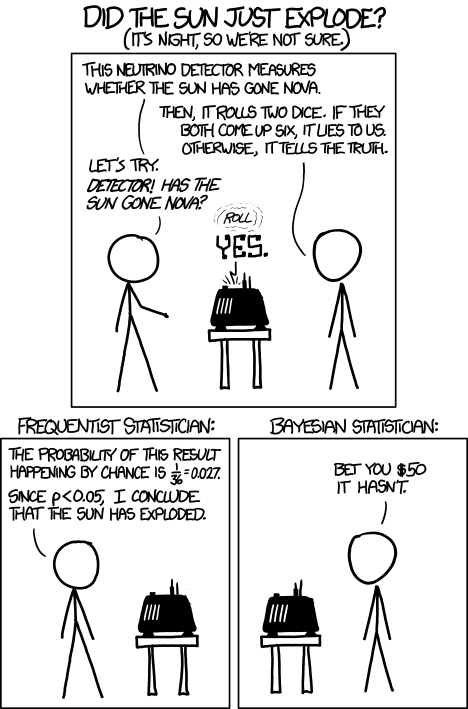
\includegraphics[width=0.4\textwidth]{images/xkcd.png} \\
Credit: Randall Monroe, xkcd
\end{center}

\end{frame}

\begin{frame}
\begin{center}
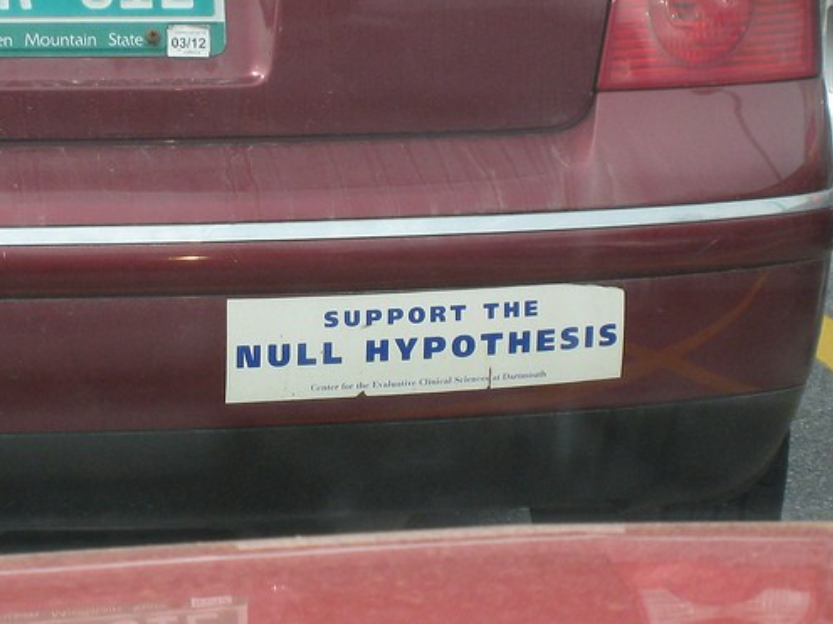
\includegraphics[width=0.6\textwidth]{images/support_null.png} \\
Credit: Unknown
\end{center}

\end{frame}

\begin{frame}
\begin{center}
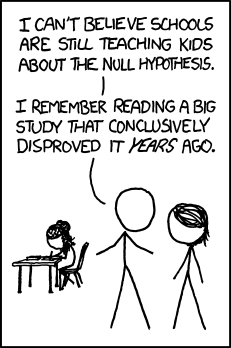
\includegraphics[width=0.4\textwidth]{images/null_hypothesis.png} \\
Credit: Randall Monroe, xkcd
\end{center}

\end{frame}


\begin{frame}
\frametitle{A Hypothesis Testing Scenario}
What if we considered these two hypotheses, as statisticians often do:
\begin{align}
H_0: \theta = 0.5 \\
H_1: \theta \neq 0.5
\end{align}
\pause

There might be a good reason to suspect the `null hypothesis' is true ---
e.g. if the effect being studied is absent.\pause

Classical/frequentist statistics would use {\bf p-values} for this, but we
will not.
\end{frame}


\begin{frame}
\frametitle{Hypothesis Testing vs. Parameter Estimation}
When we write down a list of hypotheses and get their
posterior probabilities (e.g., in a Bayes' Box), we have tested all of the
hypotheses using the data. So there is not much else to do.
\pause
\begin{itemize}
\item In classical statistics, estimation and hypothesis testing
are quite distinct and are approached using different techniques.\pause
\item For us, they're basically the same thing --- except sometimes we will use a
different prior.
\end{itemize}

\end{frame}


\begin{frame}
\frametitle{Ed Jaynes Quote}

    \begin{columns} % Create two columns
        \column{0.5\textwidth} % Left column (50% width)
        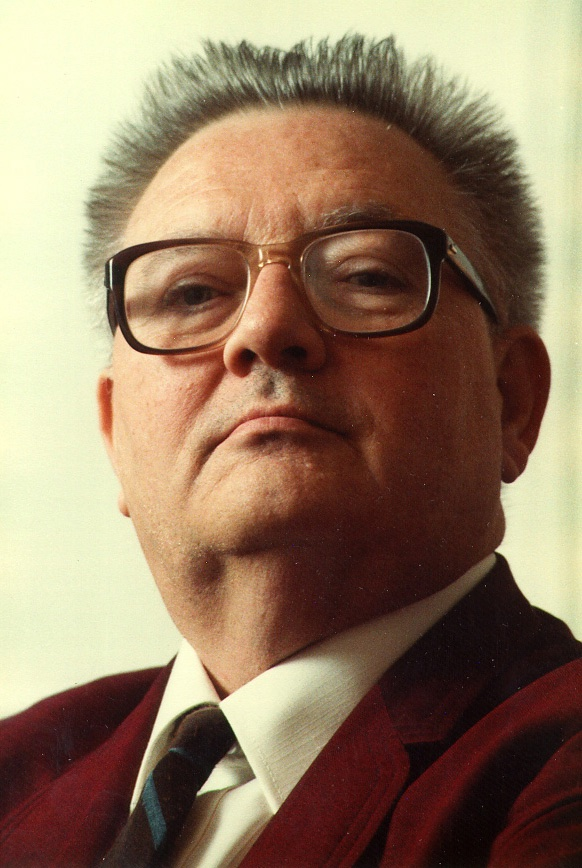
\includegraphics[width=0.7\linewidth]{images/jaynes.jpg}

        \column{0.5\textwidth} % Right column (50% width)
        {\em ``Any hypothesis testing
procedure can be
replaced by a parameter
estimation procedure that
is simpler and more
informative.''}
     \end{columns}

\end{frame}

\end{document}

